\documentclass{article}
\usepackage[utf8]{inputenc}
\usepackage[margin=1in,includefoot]{geometry}

% Header and Footer Setup
\usepackage{fancyhdr}
\pagestyle{fancy}
\fancyhead{}
\fancyfoot{}
\fancyfoot[R]{\thepage}
\renewcommand{\headrulewidth}{0pt}
\renewcommand{\footrulewidth}{0pt}
%
%Graphics Setup
\usepackage{graphicx}
\usepackage{float}
\usepackage{subfig}

%list setup
\usepackage{amssymb}
\renewcommand{\labelitemi}{$\blacktriangleright$}
\renewcommand{\labelitemii}{$\bullet$}
\renewcommand{\labelitemiii}{$\circ$}

%Source Code setup
\usepackage{xcolor}
\usepackage{listings}

\definecolor{mGreen}{rgb}{0,0.6,0}
\definecolor{mGray}{rgb}{0.5,0.5,0.5}
\definecolor{mPurple}{rgb}{0.58,0,0.82}
\definecolor{backgroundColour}{rgb}{0.95,0.95,0.92}

\lstdefinestyle{CStyle}{
    backgroundcolor=\color{backgroundColour},   
    commentstyle=\color{mGreen},
    keywordstyle=\color{magenta},
    numberstyle=\tiny\color{mGray},
    stringstyle=\color{mPurple},
    basicstyle=\footnotesize,
    breakatwhitespace=false,         
    breaklines=true,                 
    captionpos=b,                    
    keepspaces=true,                 
    numbers=left,                    
    numbersep=5pt,                  
    showspaces=false,                
    showstringspaces=false,
    showtabs=false,                  
    tabsize=2,
    language=C
}
%


\begin{document}

\begin{titlepage}

	\begin{flushright}
	\textsc{\large April 5, 2021} \\
	\end{flushright}
	\begin{center}
	\Large{\bfseries GTU Department of Computer Engineering \\ CSE312/CSE504 - Spring 2021 \\ Homework 1 Report(README)  } \\
	\end{center}
	\topskip0pt
	\vspace*{\fill}
	\begin{center}
	\Large{\bfseries Akif Kartal \\ 171044098 }
	\end{center}
	\vspace*{\fill}

\end{titlepage}

\cleardoublepage
\section{System Requirements}
In order to run spim you need to install followings;
\begin{itemize}
	\item Flex and Bison.
	\item include exceptions.s fie to the "usr/share/spim" directory.
\end{itemize}

\section{Running Spim}
\textbf{Note:} I provide the makefile with source codes if you use it, it will compile both spim and shell.c file, therefore you don't have to use it.\\
\textbf{Note:} While creating shell.asm file \textbf{I didn't use online mips compiler} since it produces very complex mips assembly code which is difficult to deal with it. Instead, I created shell.asm file myself by converting C code line by line into mips assembly very carefully and by using create process syscall.\\ \\
You can run shell based program in 3 different ways;
\begin{itemize}
	\item Compile shell.c then run "./shell". After that write "./spim -file shellHelp.asm" and hit enter.
	\item run "./spim -file shell.asm" (mips assembly version of shell.c file).
	\item run "./spim -file shellHelp.asm" (helper file to run shell.asm in spim).
\end{itemize}
\subsection{Running asm files in spim}
In order to run .asm file by using my shell after doing one of above just type filename.asm
For example;\\
run "./spim -file shellHelp.asm" then type BubbleSort.asm \\ \\
In order to create process \textbf{context switching} was made by using some memory handling codes from mem.cpp file in spim source code. \\ \\
In order to stop shell just type \textbf{exit}.\\ \\
A simple \textbf{test result} is following;
\begin{figure}[H]
    \centering
	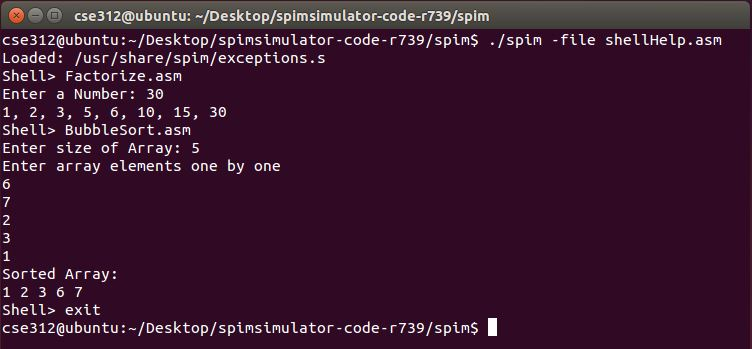
\includegraphics[width=6in, height=2.7in]{res.JPG}
	\caption[Optional caption]{}
	\label{}
\end{figure}                              

\end{document}